\section{Ergebnisse und Diskussion}
\label{sec:ergebnisseUndDiskussion}
Im nachfolgenden Kapitel werden im ersten Schritt die Ergebnisse der Datenerhebungsmaßnahmen ausgewertet und graphisch aufbereitet. Im zweiten Schritt werden die aufbereiteten Daten interpretiert, diskutiert und miteinander in Bezug gesetzt werden. Als letzten Schritt werden die Hypothesen sowie die Forschungsfrage erneut aufgegriffen und mit Hilfe der gewonnen Erkenntnisse überprüft und beantwortet.  

%%%%%%%%%%%%%%%%%%%%%%%%%%%%%%%%%%%%%%%%%%%%%%%%%%%%%%%%%%%%%%%%%%%%%%%%%%%%

\subsection{Auswertung der Logfiles}
\label{sec:auswertungDerLogfiles}
Die Daten der erhobenen Logfiles befinden sich im Ausgangszustand in einer Oracle Datenbank und können von da aus weiter verarbeitet werden. Um einen ersten Eindruck über die Daten zu bekommen, wurden bereits während der Erhebungen Datenbankabfragen entwickelt mit denen Datensätze aggregiert werden können. Dadurch konnte frühzeitig sichergestellt werden, dass die Daten ohne Probleme und in zufriedenstellender Form gesammelt und gespeichert werden. Unversehrte Daten sind für die nachfolgenden Auswertungsschritte die wichtigste Voraussetzung.

Für genauere Auswertungen wurde die Beobachtung der Logfile-Daten mit Hinblick auf die Ziele der Arbeit fokussiert. Zu Anfang soll sich bewusst erst auf die aufgestellten Kriterien und Metriken bezogen werden. In einem zweiten Schritt sollen Auffälligkeiten genauer analysiert werden und mögliche Zusammenhänge hinterfragt werden.

\textbf{Bearbeitungszeiten}

Einer der Kriterien, die im Zuge des direkten Vergleichs zwischen dem alten und neuen Dialog aufgegriffen werden sollen, ist die Bearbeitungszeit. Die Bearbeitungszeit ist die Zeit, die ein Sachbearbeiter benötigt, um ein Vermögensverzeichnis in die Cosima Oberfläche einzugeben und anschließend erfolgreich zu speichern. Bedeutet auf der anderen Seite, dass Vorgänge bei denen Sachbearbeiter den Dialog nach Eingabe von Daten ohne zu speichern schließen oder den Dialog öffnen, jedoch keine Daten eingeben, nicht einbezogen werden. Damit eine Aussage über die Bearbeitungszeit getroffen werden kann, müssen vergleichbare Daten zugrunde liegen. Dafür benötigt es eine geeignete Aggregation der Datensätze. Die aggregierten Daten zum alten sowie neuen Dialog sind im Anhang \ref{sec:datentabelleAlterDialog} und \ref{sec:datentabelleNeuerDialog} zu finden.

Der erste Schritt der Datenaggregation sieht vor, nach Art des Dialogs (alt oder neu) zu unterscheiden. Dafür dient das am Session-Objekt hängende Attribut \enquote{DialogID}. Als zweiter Schritt werden die Sessions herausgefiltert, die eine Speicherung der Daten beinhalten. Dazu sollen auch nur die Sessions genutzt werden bei denen mindestens eine Veränderung der Daten stattgefunden hat. Das alleinige Öffnen des Dialogs zum Einsehen von Informationen wird nicht gewertet. Für die Einhaltung der aufgestellten Bedingungen werden die beiden Attribute \enquote{WertGeaendertFlag} und \enquote{GespeichertFlag} genutzt. Durch die Flags lässt sich zum einen erkennen, ob das Bedienelement, auf dem die Interaktion stattgefunden hat, eine Veränderung erfahren hat oder nicht. Zum anderen wird hinterlegt, ob die veränderten Daten gespeichert wurden.

Alle Sessions, die den oben aufgestellten Bedingungen entsprechen, gehören zu den gesuchten Bearbeitungsvorgängen. Die Vorgänge werden in einem weiteren Schritt auf einzelne Tage gruppiert. Es lässt sich bereits erkennen, dass die Menge der Bearbeitungsvorgänge mit dem alten Dialog, nur 15 Sessions mehr beinhaltet als die Menge der erhobenen Bearbeitungsvorgänge mit dem neuen Dialog. Für einen nachfolgend aussagekräftigen Vergleich von Durchschnittswerten, die auf Basis dieser Mengen berechnet werden, sind die beieinanderliegende Stichprobenumfänge eine gute Ausgangslage.

Mit Hilfe der Sessions-Attribute \enquote{Startzeitpunkt} und \enquote{Endzeitpunkt} können die Bearbeitungszeiten einzelner Sessions ermittelt werden und anschließend zusammengeschlossen werden, um den Mittelwert auf Tagesbasis zu berechnen. Da die resultierenden Daten vereinzelt Spitzen in den Bearbeitungszeiten aufzeigen, wird der gleitende Durchschnitt (GD) dritter Ordnung angewandt, um den Verlauf zu glätten. Ursprünglich wurden beide Dialoge jeweils über einen Zeitraum von 11 Tagen gemessen, jedoch fallen nun die ersten beiden Periodenwerte aufgrund des GD weg. Es bleiben neun Perioden für die Darstellung des zeitlichen Verlaufs der Bearbeitungszeiten. Diese sollten ausreichen, um einen Eindruck über die Entwicklung zu erhalten.

Werden nun die Bearbeitungszeit (Sekunden) gegen die Periode (Tage) in einem Diagramm aufgetragen sieht der geglättete Verlauf der durchschnittlichen Bearbeitungszeiten wie folgt aus:
\begin{figure}[H]
  \centering
  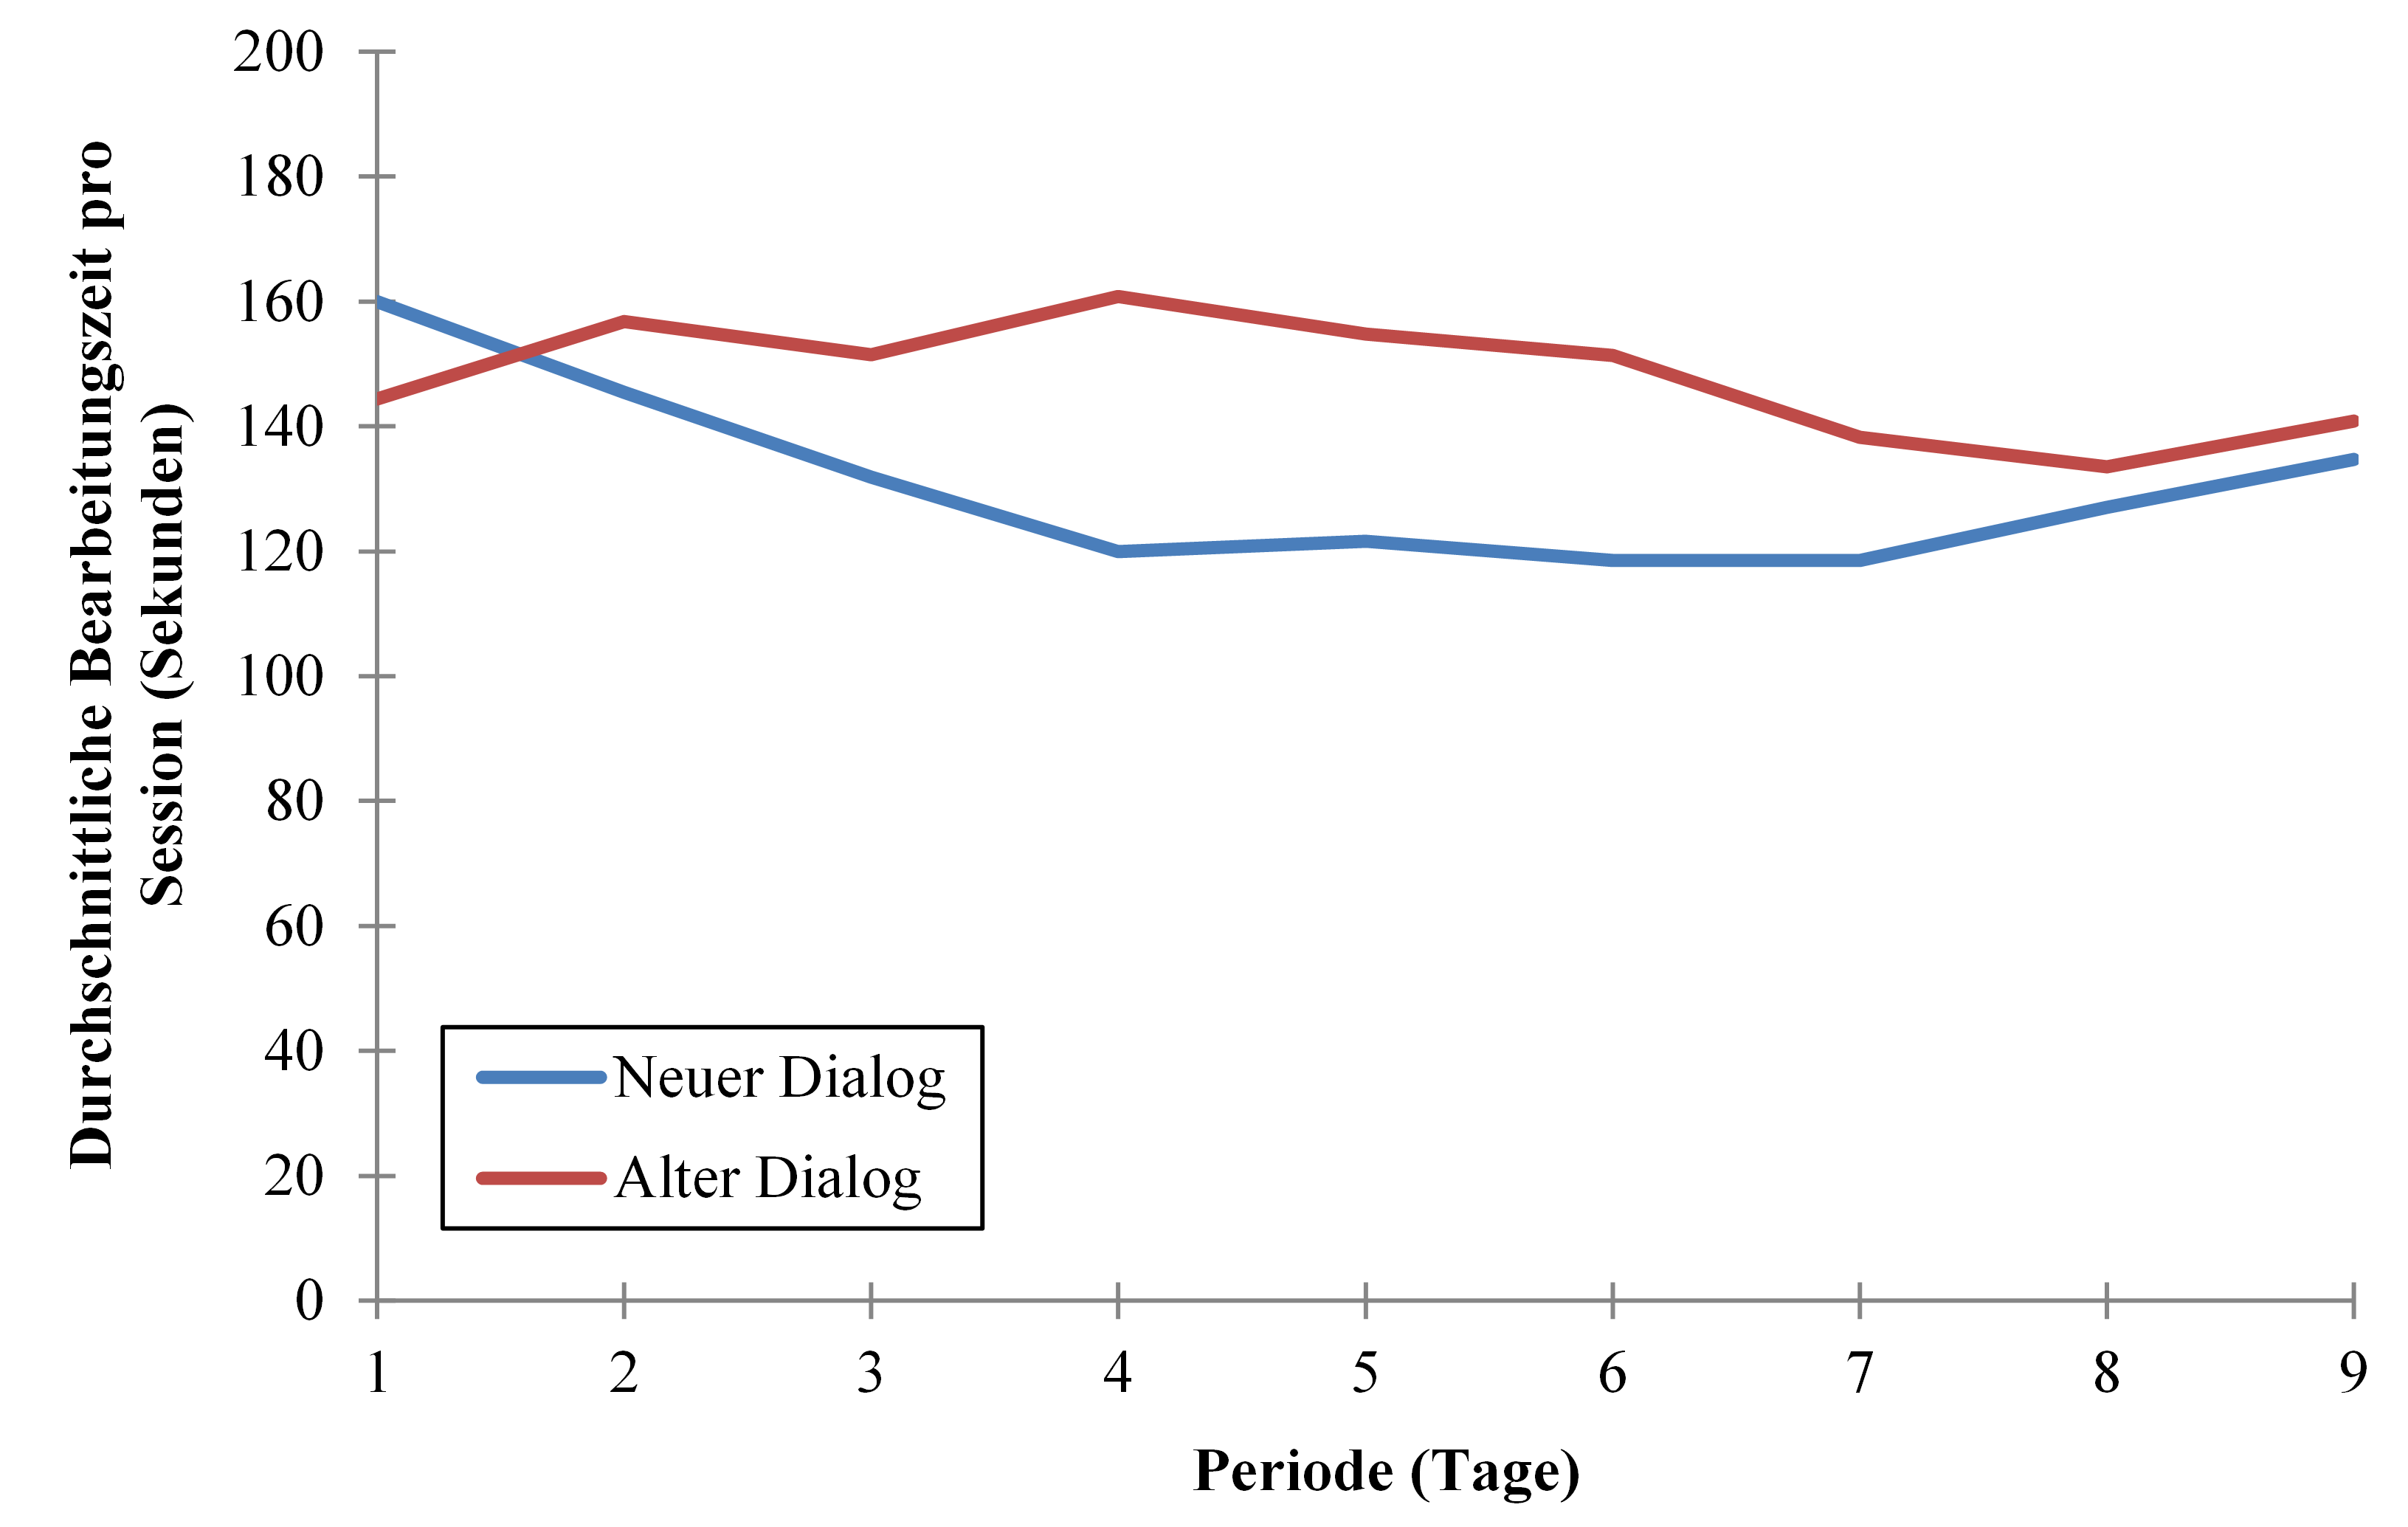
\includegraphics[]{img/Bearbeitungszeit_Verlauf.png}
  \caption{Vergleich des Verlaufs der durchschnittlichen Bearbeitungszeiten beider Dialoge.}
  \caption*{\textbf{Quelle:} Eigene Darstellung}
  \label{fig:BearbeitungszeitVerlauf}
\end{figure}
Es lässt sich erkennen, dass die durchschnittliche Bearbeitungszeit pro Session im alten Dialog (rote Linie) im Bereich von 140 Sekunden bis 160 Sekunden leicht schwankt. Zudem ist die gemittelte Bearbeitungszeit über alle Perioden mit 147 Sekunden, 14 Sekunden über der des neuen Dialogs (133 Sekunden).

Eine weitere Auffälligkeit innerhalb des Verlaufs des neuen Dialogs sind die ersten vier Perioden. In diesen sinkt die Bearbeitungszeit kontinuierlich von etwa 160 Sekunden auf durchschnittlich 120 Sekunden ab. Ab dort ist der Verlauf bis zum Ende der siebten Periode konstant. Anschließend steigt die Bearbeitungszeit wieder leicht auf 135 Sekunden an. Hingegen ist zu erkennen, dass die blaue Linie ab der zweiten Periode durchgehend unterhalb der roten Linie verläuft. Also die durchschnittliche Bearbeitungszeit im neuen Dialog, fast durchgängig geringer ist, als die im alten Dialog. Diese Tatsache sollte aber mit gewisser Vorsichtig betrachtet werden, da die Perioden, also sowohl der Wochentag als auch der anfallende Arbeitsaufwand an dem Tag, in denen die Erhebungen durchgeführt wurden nicht identisch sind.

\pagebreak
\textbf{Mausklicks und Tastaturanschläge}

Als weitere Kennzahl für den Vergleich der Dialoge, dient die Anzahl von Interaktionen insgesamt, sowie deren Unterteilung in Mausklicks und Tastaturanschläge. Hiermit sollen Hinweise gesammelt werden, die dabei helfen können eine Aussage über die Komplexität und die physische Belastung bei der Arbeit mit den Dialogen zu treffen.

Als Erstes sollen die oben bereits ermittelten Bearbeitungsvorgänge genutzt werden, um alle Interaktionen zu bekommen. Es lässt sich anschließend mit Hilfe des Interaktions-Attributs \enquote{Typ} eine Unterscheidung zwischen Maus und Tastatur treffen. In Abbildung \ref{fig:verlaufInteraktionenAlterDialog} sowie in Abbildung \ref{fig:verlaufInteraktionenNeuerDialog} wurden die Interaktionen nach Typ gestaffelt gegen die Perioden in Tagen in einem Balkendiagramm aufgetragen. Die Datentabellen mit allen Werten zu den Interaktionen beider Dialoge ist im Anhang \ref{sec:datentabelleAlterDialog} bzw. \ref{sec:datentabelleNeuerDialog} zu finden. Es ist darauf zu achten, dass Interaktionen nur in ganzzahligen Werten in der Realität existieren. Die dargestellten Mittelwerte sind jedoch Dezimalzahlen mit zwei Nachkommastellen, um die Verhältnisse genauer darzustellen.
\begin{figure}[H]
  \centering
  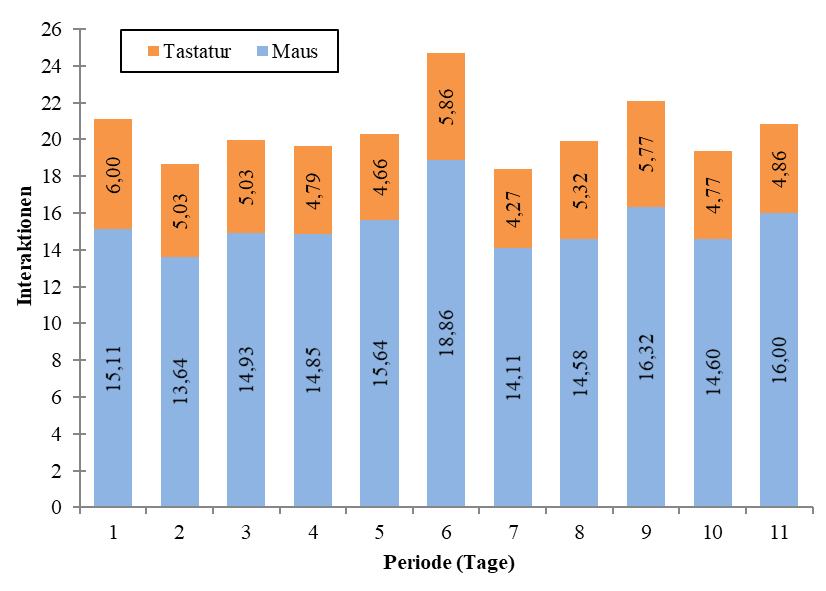
\includegraphics[]{img/Interaktionen_Alter_Dialog.png}
  \caption{Verlauf der Interaktionen im alten Dialog.}
  \caption*{\textbf{Quelle:} Eigene Darstellung}
  \label{fig:verlaufInteraktionenAlterDialog}
\end{figure}
Werden die Interaktionen pro Periode im alten Dialog betrachtet, lässt sich erkennen, dass die Werte pro Periode gerundet zwischen 18,4 und 24,7 Interaktionen schwanken. Werden Tastatur- und Maus-Interaktionen relativ zueinander erfasst, so wird die Tastatur zwischen 22,95\% und 28,42\% genutzt. Die Maus hingegen besitzt ein Maximum von 77,05\% und ein Minimum von 71,58\% an den gesamten Interaktionen einer Periode. Im Durchschnitt wird die Tastatur zu 25,06\% und die Maus zu 74,94\% verwendet.

\begin{figure}[H]
  \centering
  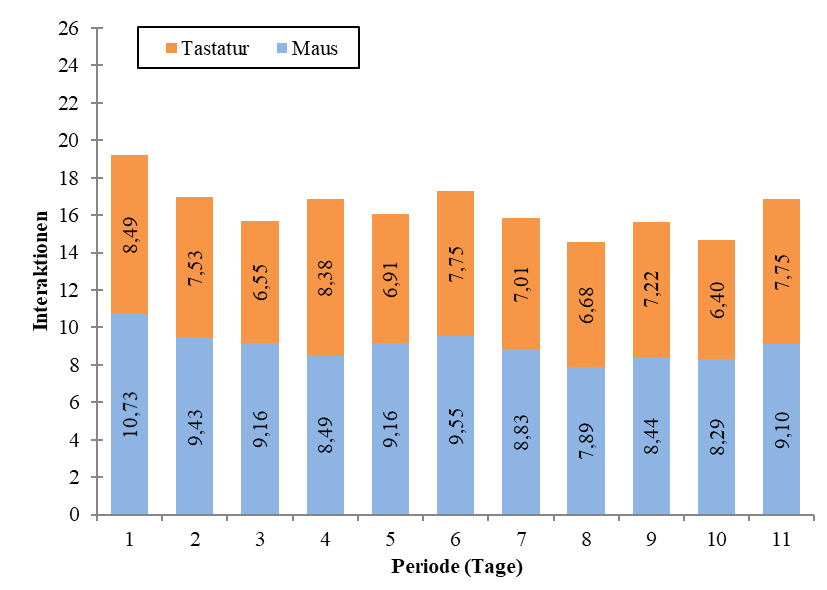
\includegraphics[]{img/Interaktionen_Neuer_Dialog.png}
  \caption{Verlauf der Interaktionen im neuen Dialog.}
  \caption*{\textbf{Quelle:} Eigene Darstellung}
  \label{fig:verlaufInteraktionenNeuerDialog}
\end{figure}
Im neuen Dialog ist zu erkennen, dass die Werte im Schnitt zwischen 14,5 und 19 Interaktionen liegen. Bei der Ermittlung von relativen Anteilen, liegt der Anteil von Tastatur-Interaktionen in einem Bereich von 41,67\% bis 49,67\%. Die anteilige Benutzung der Maus liegt zwischen 50,33\% und 58,33\%. Im Durchschnitt wird die Tastatur für 44,86\% und die Maus für 55,14\% der Interaktionen genutzt.

% Vergleich
Werden beide Dialoge miteinander verglichen so ist zum einen festzustellen, dass die Interaktionen im neuen Dialog geringere Schwankungen verzeichnen und zum anderen ist die durchschnittliche Anzahl von Interaktionen pro Session gemittelt über alle Perioden im alten Dialog etwa 25\% höher als im neuen Dialog. Zum anderen hat sich das Verhältnis von Tastatur- und Maus-Interaktionen verschoben. Mit dem neuen Dialog sind die Tastatur-Interaktionen um knapp 20\% gestiegen, dafür ist die Benutzung der Maus um 20\% zurückgegangen. Insgesamt wurden im neuen Dialog durchschnittlich pro Session knapp 4 Interaktionen weniger ausgeübt, als im alten Dialog.

\textbf{Anzahl und relative Häufigkeit von Veränderungen}

Wie bereits oben genannt wurden die Daten in zwei hintereinander liegenden Zeiträumen erhoben, in denen je nach aktuellem Aufkommen unterschiedlich viele Vorgänge mit unterschiedlichen Komplexitäten vorliegen. Die Komplexität soll im folgenden mit der Anzahl an Veränderungen bzw. den Eingaben von Daten auf der Oberfläche gleichgesetzt werden. Das heißt, umso mehr Daten einzugeben sind, desto komplexer ist die Bearbeitung des Vorgangs zu bewerten. Die Komplexität soll dabei helfen beide Stichprobenumfänge die Datengrundlage beider Dialog besser miteinander vergleichen zu können.

Um die Komplexität zu vergleichen wurde die relative Häufigkeit von Veränderungen gegen die Anzahl von Veränderungen (bis 50 Veränderungen) pro Session in einem Balkendiagramm (siehe Anhang \ref{sec:verteilungVeraenderungen}) aufgetragen. Aufgrund der Größe der Grafik wurde diese bewusst in den Anhang der Ausarbeitung verschoben. 

Der Komplexitätsvergleich wird auf der Grundlage von 777 Sessions aus dem neuen Dialog und 781 aus dem alten Dialog aufgestellt. Es fällt auf, dass die Verteilung von wenigen Veränderungen zu vielen Veränderungen innerhalb einer Session (gemessen am GD zweiter Ordnung) bei beiden Dialogen unterschiedlich aussieht. Der neue Dialog hat einen größeren Anteil von weniger komplexen Sessions (5 bis 13 Veränderungen). Im alten Dialog wiederum ist der Großteil der Sessions im Bereich von 11 bis 22 Veränderungen angesiedelt. Ab 35 Veränderungen ähneln sich beide Graphen wieder relativ stark. 

%%%%%%%%%%%%%%%%%%%%%%%%%%%%%%%%%%%%%%%%%%%%%%%%%%%%%%%%%%%%%%%%%%%%%%%%%%%%

\subsection{Auswertung der Fragebögen}
\label{sec:auswertungDerFrageboegen}
Für die Auswertung der Fragebögen, die im Kapitel \ref{sec:durchfuehrungEvaluation} von den Probanden erhoben wurden, werden alle Datensätze in eine Excel-Tabelle übertragen. Daraufhin werden die Daten so angeordnet, dass jede Zeile einem Bewertungsaspekt aus dem ISO Fragebogen entspricht (siehe Abb. \ref{fig:auswertungsmatrixNeuerDialog} und Anhang \ref{sec:auswertungsmatrixAlterDialog}). Die Ausprägungen für die Bewertung eines Items werden so formatiert, dass sie anstatt von \enquote{$---$} bis \enquote{$+++$} den Werten von -3 (sehr negativ) bis +3 (sehr positiv) entsprechen. Dies hat den Vorteil das anschließend mit den numerischen Werten weiter gerechnet werden kann, da sie ein repräsentatives Abbild der Antworten darstellen und der Ordnung der Likert-Skala entsprechen\footnote{\cite[vgl.][]{Statista}}. Zudem wurden die Kennzahlen in den Auswertungsmatrizen farblich hinterlegt, damit zwischen negativen (rot) und positiven (grün) Bewertungen unterschieden werden kann. Das Rating der 35 Bewertungsaspekte wurde mit Hilfe der Mittelwerte aus den Bewertungen aller Teilnehmer berechnet. Die Benutzerzufriedenheit eines Gestaltungsgrundsatz wird ebenfalls durch den Mittelwert der fünf zuvor berechneten Mittelwerte der Bewertungsaspekte gebildet und besitzt anschließend einen Wert zwischen -3 und +3. Aus Darstellungsgründen wurden die Zahlen im Folgenden alle auf drei Stellen nach dem Komma gerundet.

In Abbildung \ref{fig:auswertungsmatrixNeuerDialog} sind alle Einschätzungen zu dem neuen Vermögensverzeichnis Dialog in aggregierter Form dargestellt. Stellt man diese Auswertungsmatrix in einen direkten Vergleich zu den Auswertungen des alten Dialogs (siehe Anhang \ref{sec:auswertungsmatrixAlterDialog}) lässt sich erkennen, dass der neue Dialog in allen sieben Gestaltungsgrundsätzen besser bewertet wurde, als der alte Dialog (siehe Abb. \ref{fig:vergleichBalkendiagramm}). 
\begin{figure}[H]
  \centering
  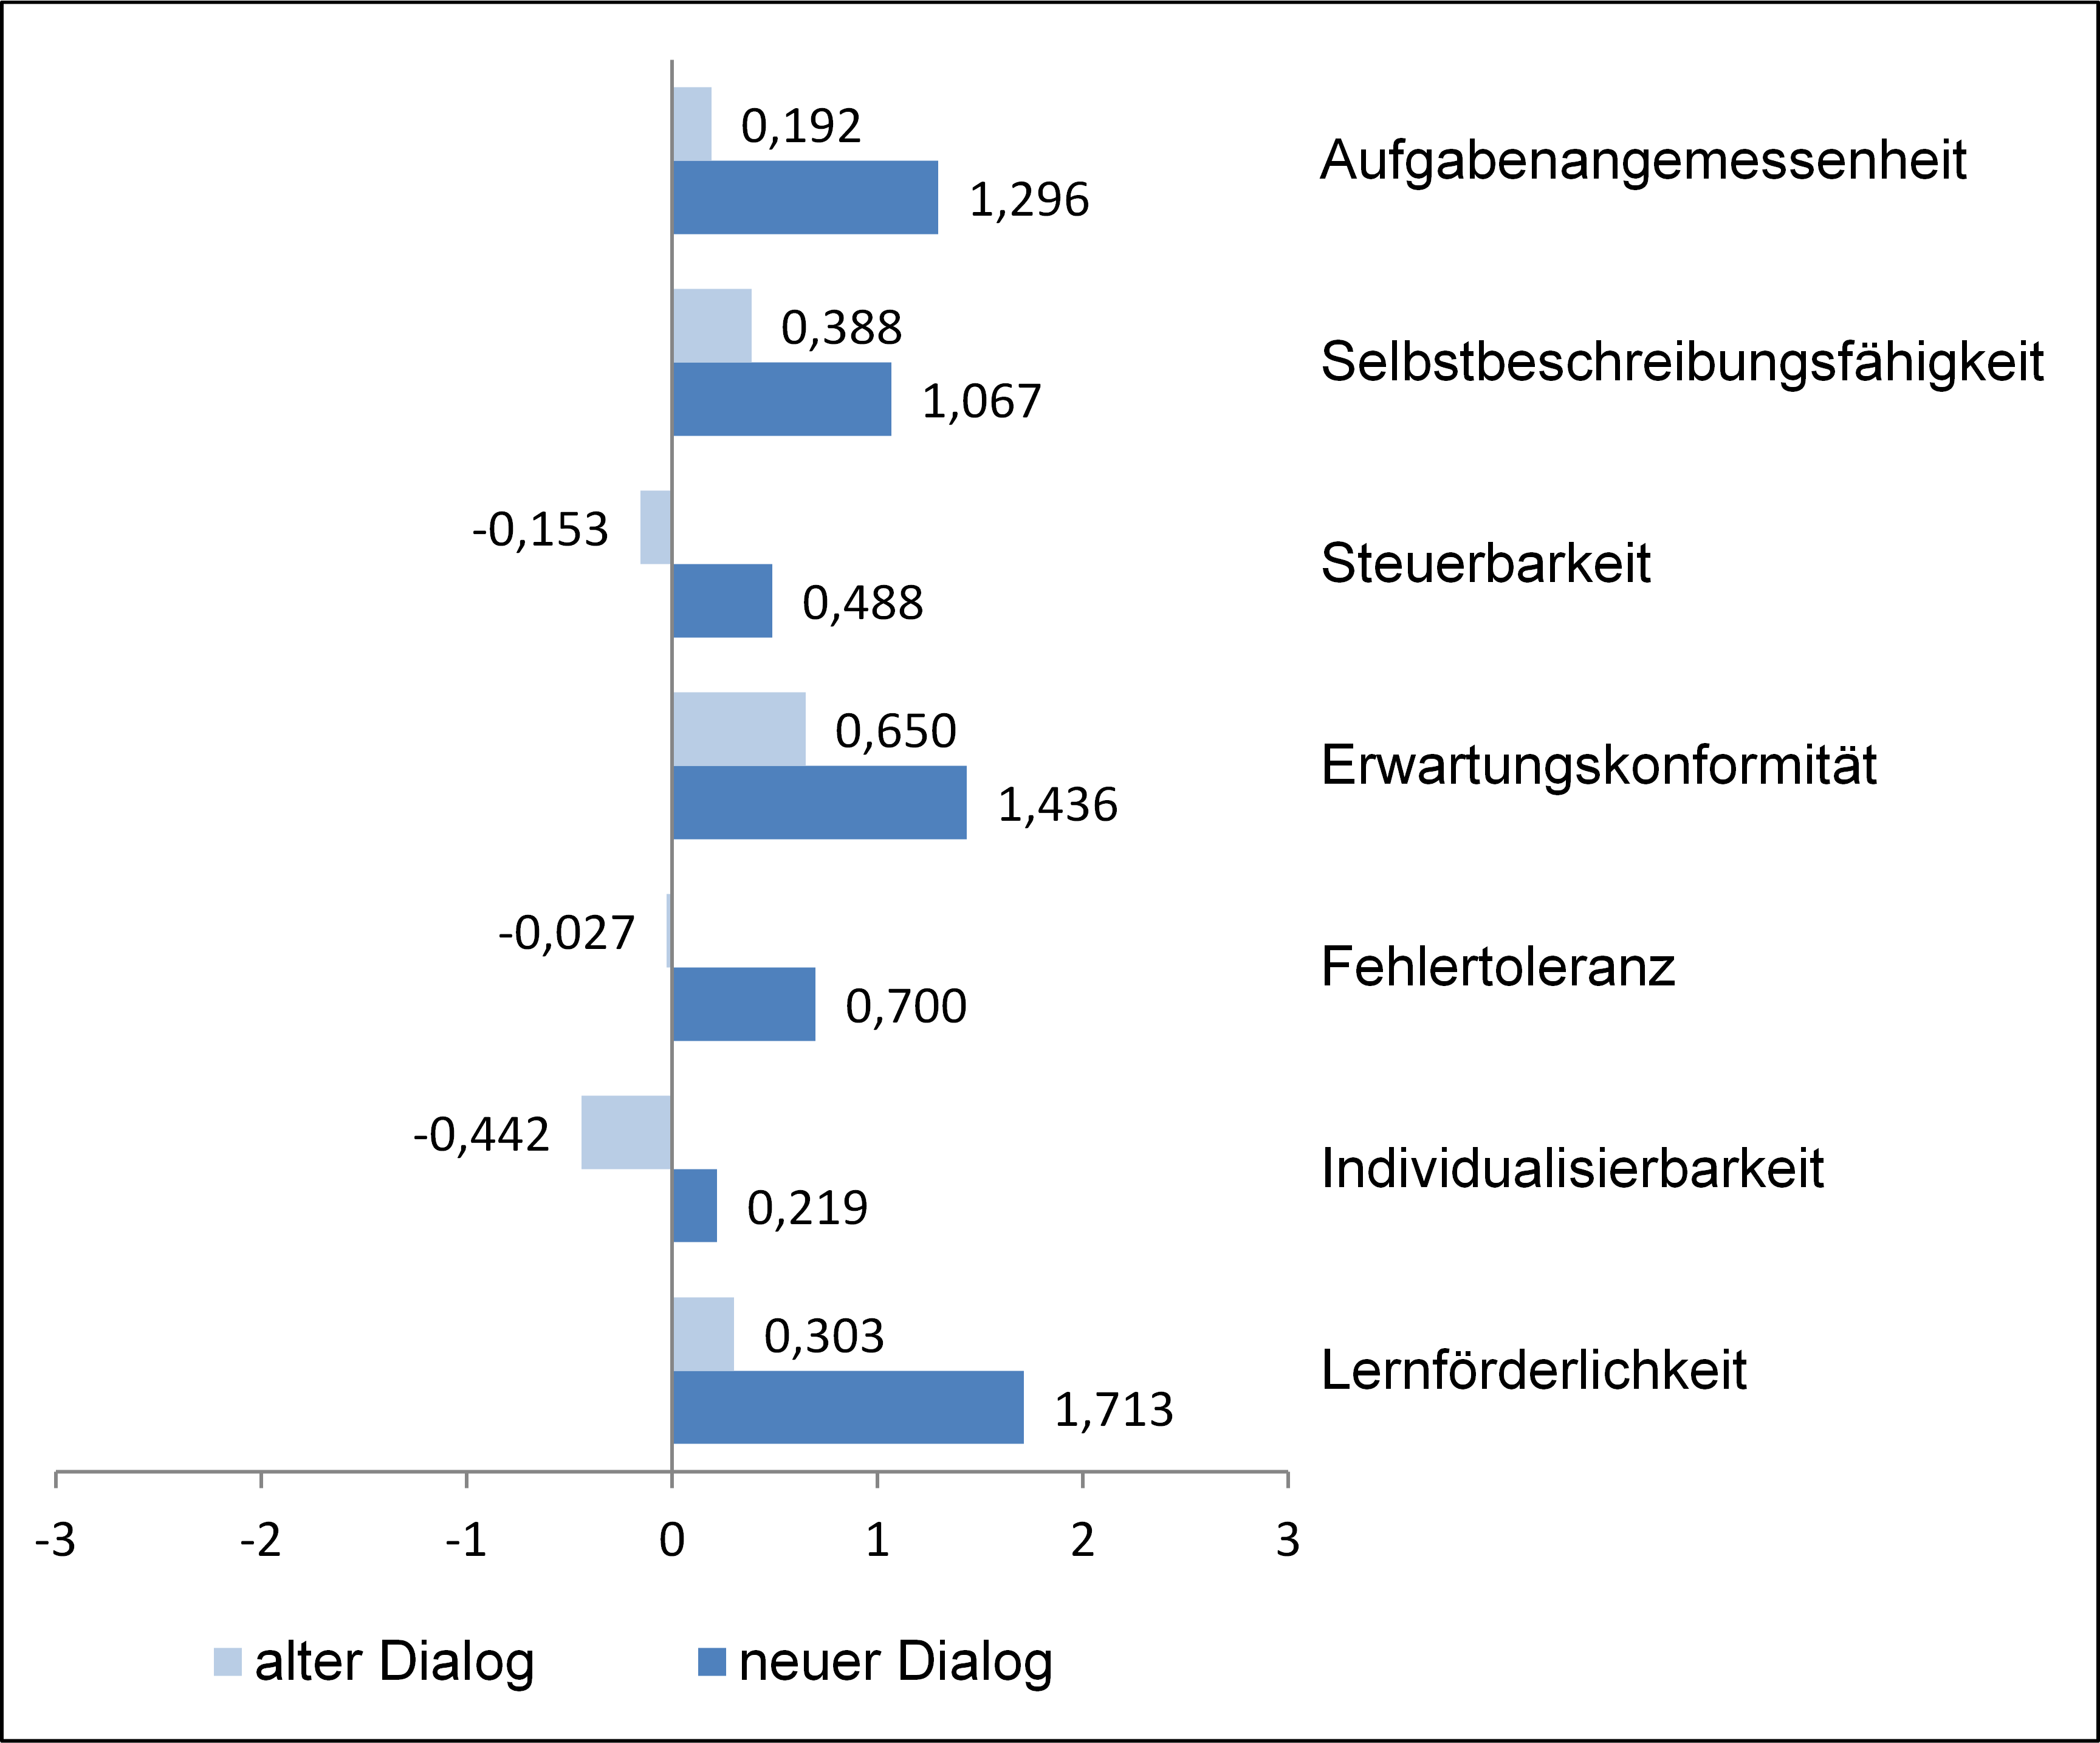
\includegraphics[scale=0.88]{img/ISO9241-10_Vergleich_Balkendiagramm.PNG}
  \caption{Vergleich der Gestaltungsgrundsätze zwischen altem und neuen Dialog.}
  \caption*{\textbf{Quelle:} Eigene Darstellung}
  \label{fig:vergleichBalkendiagramm}
\end{figure}
Die größte Steigerung kann in den Gebieten Aufgabenangemessenheit und Lernförderlichkeit mit 1,1 Punkten und 1,4 Punkten verzeichnet werden. Am wenigsten konnte die Benutzerzufriedenheit bei der Steuerbarkeit und der Individualisierbarkeit steigen. 

Trotz der insgesamt positiven Ergebnisse, gibt es immer noch Bereiche in denen die Bewertungen eher schwach ausfallen. Dazu zählt auch die Steuerbarkeit des Dialogs. Diese ist zwar positiv, also bietet ausreichend Freiheit bei der Bedienung, jedoch empfinden die Benutzer die Unterbrechungsfreiheit und die Anpassbarkeit von Informationsdarstellungen noch nicht vollkommen zufriedenstellend. Dieses Thema ist eher komplex zu bewerten, da hier auf die einzelnen Wünsche und Belangen der einzelnen Sachbearbeiter eingegangen werden müsste, um weitere Verbesserungen zu erzielen.

Auch die Kategorie Individualisierbarkeit selbst konnte im direkten Vergleich einen Gewinn von knapp 0,7 Punkte verzeichnen. Jedoch liegt die Bewertung mit +0,219 im unteren positiven Bereich. Besonders die Punkte \enquote{Erweiterbarkeit durch den Benutzer} und \enquote{Individuelle Anpassbarkeit durch den Benutzer} fallen beide noch schlecht aus. Gleichzeitig sind die beiden Bewertungsaspekte, trotz ihres Anstiegs um 0,4 bzw. 0,6 Punkten, auch die einzigen die noch negativ bewertet wurden. Sie spiegeln die individuelle Erweiterbarkeit und Anpassbarkeit von Bearbeitungsschritte und Benutzer wider. Die Kritik an dieser Stelle ist aber durchaus nachzuvollziehen, da sich der Dialog nur an wenigen Stellen individuell anpassen lässt. Ein Grund dafür ist die niedrige Priorisierung von individuellen und dynamischen Strukturen während der Konzeptionsphase. Es ist denkbar in einem nachfolgenden Projekt noch einmal explizit auf die beiden Aspekte und Benutzeranliegen einzugehen, um bestenfalls die Benutzerzufriedenheit weiter zu verbessern.

Insgesamt ist die Selbstbeschreibungsfähigkeit mit einem Wert von +1,067 durchaus zufriedenstellend. In Bezug auf die, durch den Benutzer geforderten und die durch das System automatisierten Erklärungen, ist aber noch klar ein Verbesserungspotential zu erkennen. Hier könnten gezielte Maßnahmen eingeleitet werden, bei denen zusammen mit dem Fachbereich fehlende Erklärungen evaluiert und anschließend ergänzt werden. Dies sollte einen vergleichsweise geringen Aufwand darstellen und kann auf der anderen Seite große Effekte erzielen.

Mit dem Blick auf die positiven Eigenschaften des neuen Vermögensverzeichnis Dialogs fallen unter die besten fünf Punkte:
\begin{enumerate}
    \setlength{\itemsep}{0pt}
    \setlength{\parskip}{3pt}
    \setlength{\parsep}{2pt}
    \item Hilfe beim Behalten von Gelerntem (+2,104),
    \item Autodidaktisch\footnote{Autodidaktisch = Wissen durch Literatur, Übungen, Beobachtungen oder Versuche eigenständig aneignen } (+2,085),
    \item Bedienungskomplexität (+2,083),
    \item Zeit für Einarbeitung (+2,063) und
    \item Erfordernis, sich Details zu merken (+1,979).
\end{enumerate}
Interessant ist, dass vier der fünf Punkte aus dem Bereich Lernförderlichkeit stammen. Der Aspekt \enquote{Bedienungskomplexität} wiederum gehört zum Grundsatz Aufgabenangemessenheit. Hier bewerten die Benutzer die Bedienung des neuen Dialogs, mit einem durchschnittlichen Schwellwert von etwa +2, als angenehm und einfach. Im Vergleich ist dies ein Anstieg von über 1,6 Punkten. Die gestiegene Benutzerzufriedenheit von über 1,4 Punkten im Bereich der Lernförderlichkeit kann genauso wie die Bedienungskomplexität durch die Vereinfachung und Verringerung von Informationen, Bedienelementen und Strukturen erklärt werden. 
\begin{figure}[H]
  \centering
  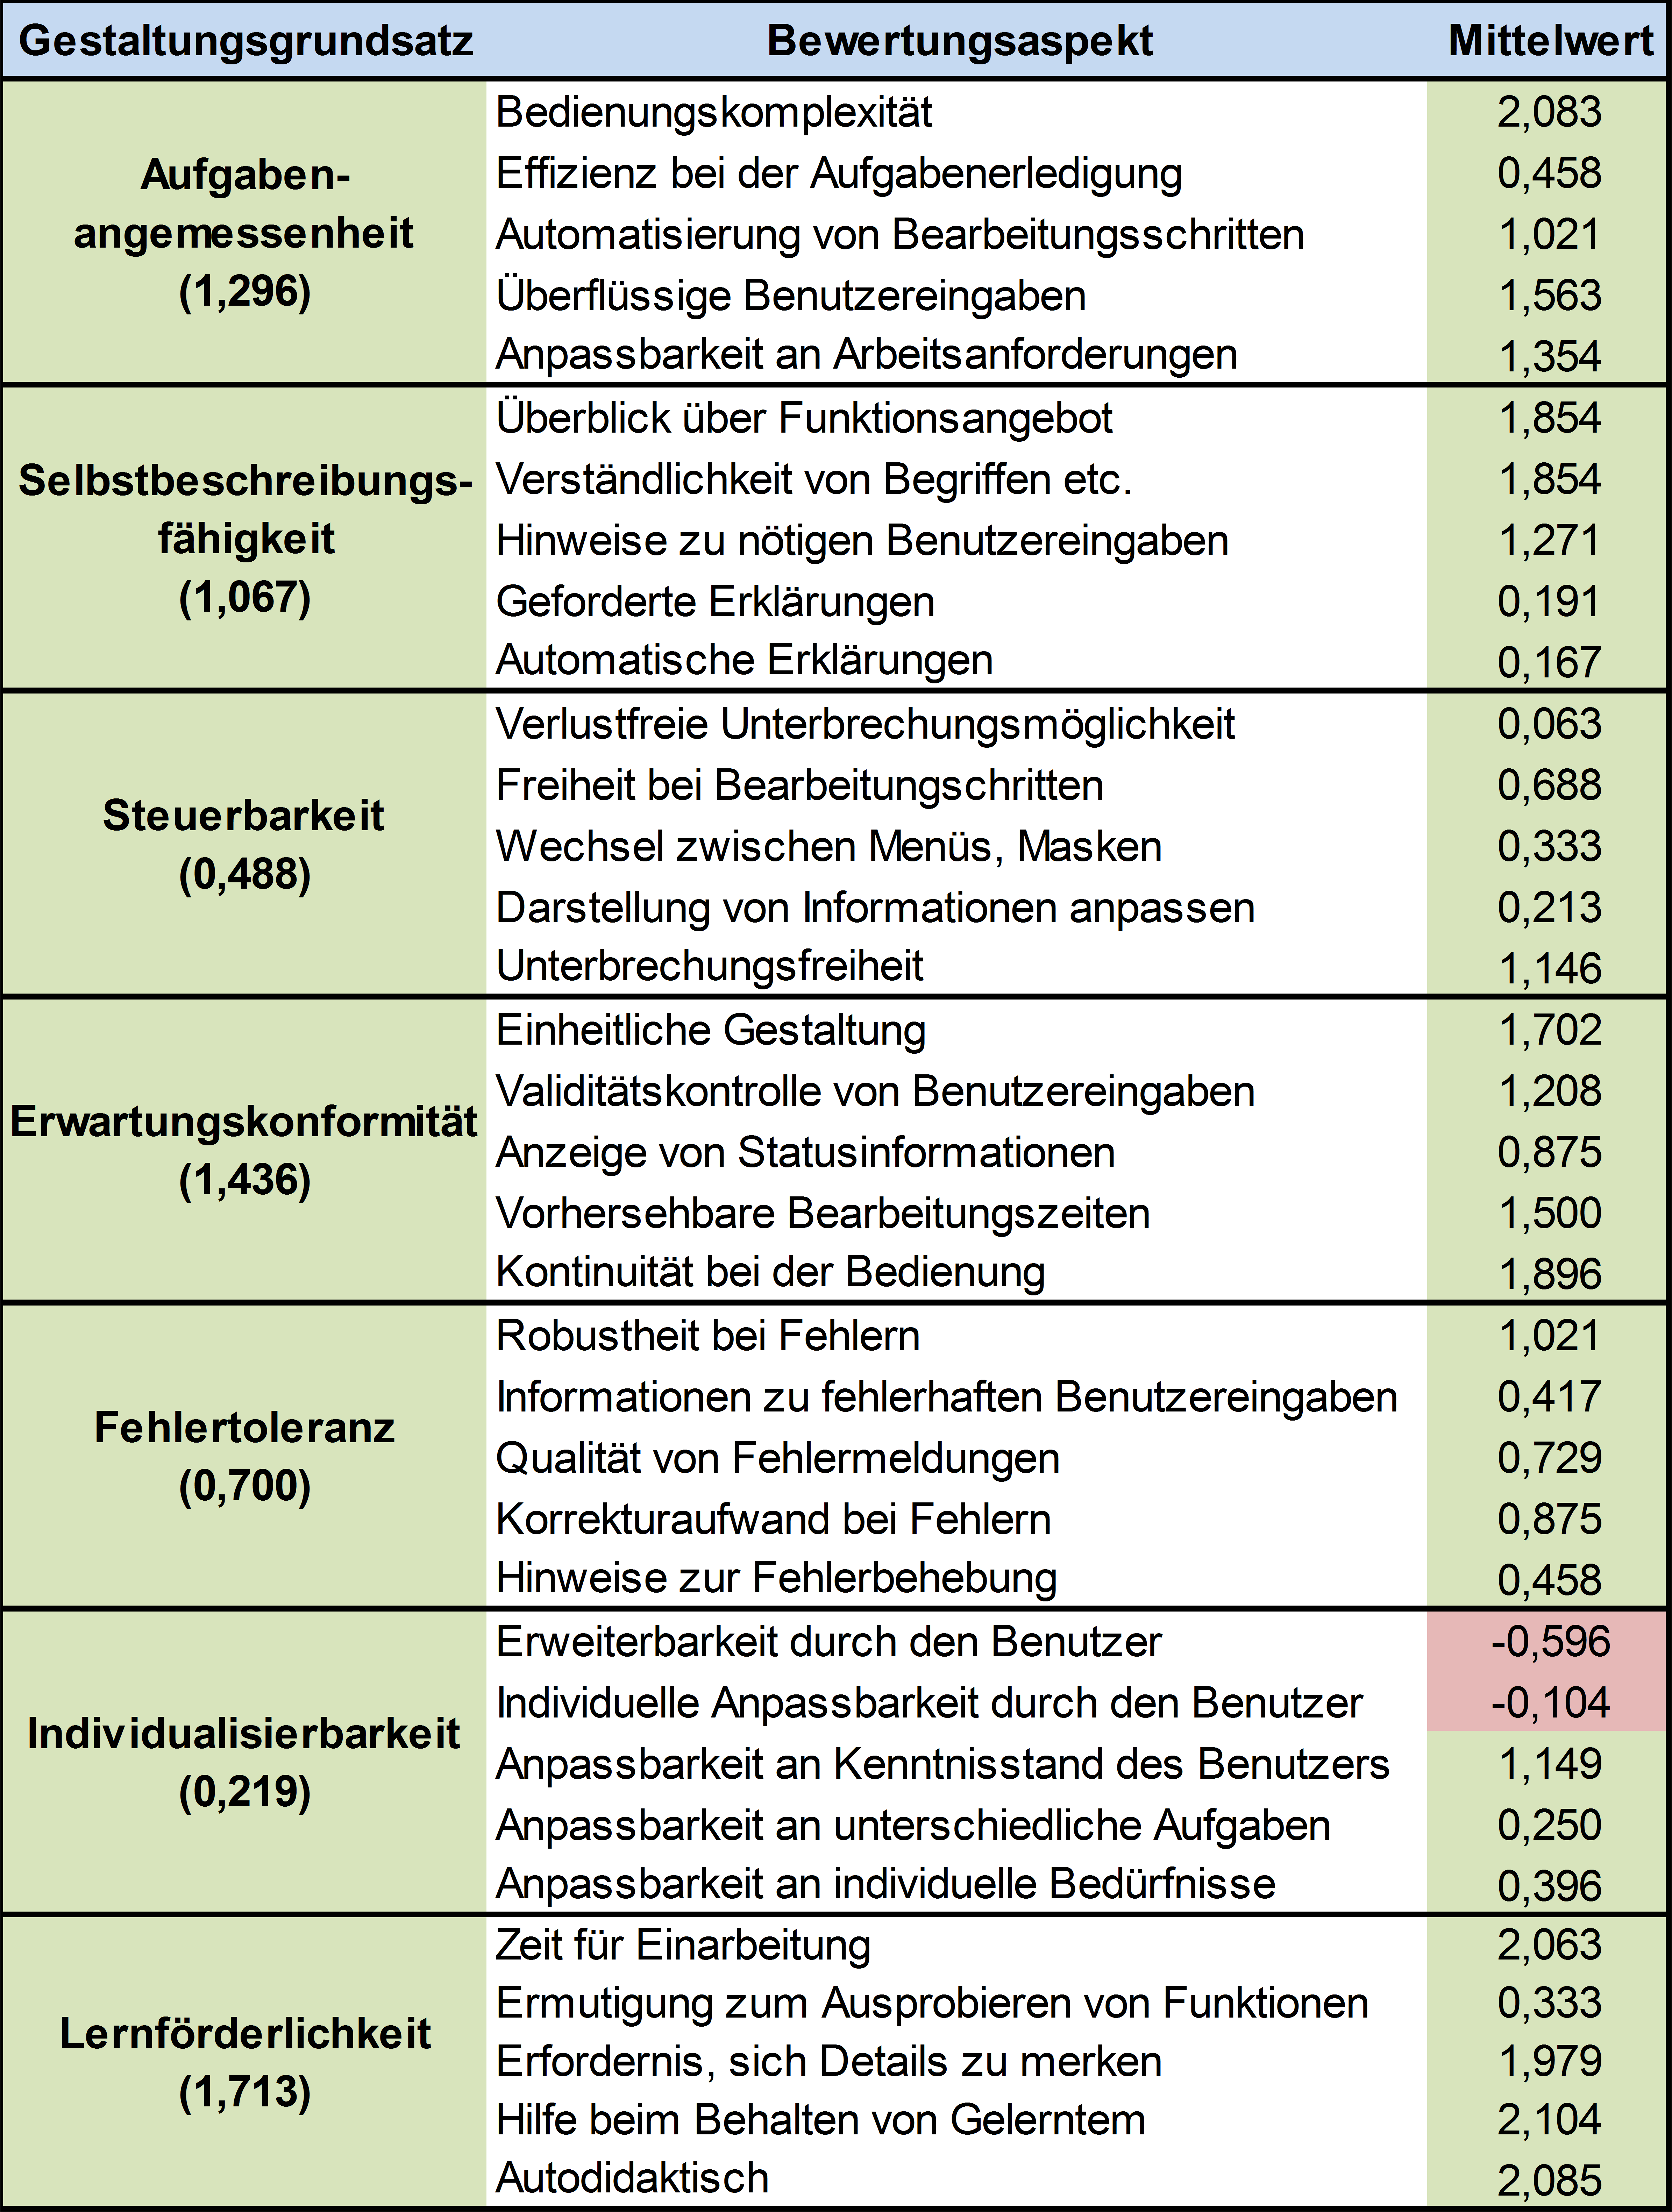
\includegraphics[width=400px]{img/Auswertungsmatrix_Neuer_Dialog.PNG}
  \caption{Auswertungsmatrix zum ISO 9241-10 Fragebogen neuer Dialog.}
  \caption*{\textbf{Quelle:} Eigene Darstellung}
  \label{fig:auswertungsmatrixNeuerDialog}
\end{figure}
Die fünf Bewertungsaspekte sollten gerade mit Blick auf die Zeit positive Auswirkungen haben. Fällt die Betrachtung auf die Punkte zwei und vier so lässt sich ableiten, dass potentiell künftig Zeit eingespart werden kann. Es muss sich lediglich der Anwendungsfall \enquote{Neuer Mitarbeiter} vorgestellt werden. Der neue Mitarbeiter benötigt tendenziell weniger Zeit für die Einarbeitung in den neuen Dialog. Zudem kann der zeitliche Aufwand für helfende und einweisende Kollegen verringert werden.

So lassen sich auch die Punkte \enquote{Erfordernis, sich Details zu merken} und \enquote{Hilfe beim Behalten von Gelerntem} mit einer gesteigerten Effizienz in Verbindung bringen. Ein möglicher Anwendungsfall hierfür ist ein Vermögensverzeichnis, das viele Details enthält. Hier muss der Sachbearbeiter im Gegensatz zum alten Dialog nur noch einen Bruchteil der Informationen übernehmen und somit auch weniger Informationen gleichzeitig im Gedächtnis behalten. Dies kann durchaus positive Effekte auf die Bearbeitungszeit und die mentale Belastung des Sachbearbeiters nehmen.

Im Gesamtüberblick kann bereits ein positiver Verlauf der Benutzerzufriedenheit in allen sieben Grundsätzen verzeichnet werden. Hieraus lässt sich bereits auf eine gewisse Effektivität des Projekts schließen, besonders mit Bezug auf die zeitlichen Effekte. Die Benutzer scheinen allgemein zufriedener bei der Arbeit mit dem neuen Dialog.

%%%%%%%%%%%%%%%%%%%%%%%%%%%%%%%%%%%%%%%%%%%%%%%%%%%%%%%%%%%%%%%%%%%%%%%%%%%%

\subsection{Abschließende Ergebnisdiskussion}
\label{sec:abschliessendeErgebnisdiskussion}
Im letzten Schritt werden die gesammelten Erkenntnisse zusammengefasst und in einen Zusammenhang gebracht. Zusätzlich werden die Ergebnisse mit weiteren Argumenten und verschiedenen Blickrichtungen angereichert, um abschließend die drei Hypothesen H1\textsubscript{0}, H2\textsubscript{0} und H3\textsubscript{0} zu belegen bzw. zu widerlegen. Das Ziel ist es ein abschließendes Ergebnis für die Evaluation bzw. die Zielerreichung der Abschlussarbeit zu erhalten.

% Hypothese H1
Hinsichtlich der ersten Hypothese H1\textsubscript{0} ist mit den vorliegenden Fakten und Annahmen zu überprüfen, ob diese belegt werden kann oder nicht. Werden Argumente gesucht und vorliegende Erkenntnisse verwendet, um die Nullhypothese zu widerlegen, so könnte argumentiert werden, dass aufgrund der Verteilung von Veränderungen, die bereits in der Logfile-Auswertung dargelegt wurde, eine höhere Komplexität im Testzeitraum des alten Dialogs vorlag. Somit ist davon auszugehen, dass eine höhere Komplexität auch zu einer erhöhten Bearbeitungszeit geführt haben könnte. Auf der anderen Seite kann diese Kontra Argument auch in gewisse Weise relativiert werden, da die gemessene Komplexität nur die Anzahl von Veränderungen misst und nicht spezifisch die Art der Veränderungen mit einbezieht. Das heißt eine Vielzahl von Veränderungen, die lediglich das Anklicken von Checkboxen beinhalten, sind nicht unbedingt komplexer einzuschätzen als wenige Änderungen, die das Ausfüllen von Textfeldern benötigen. Über die genaue Komplexität lässt sich mit den vorliegenden Auswertungen keine eindeutige Auskunft geben. Ein weiterer Fakt, der gegen die Nullhypothese spricht ist, dass in beiden Erhebungszeiträumen nicht die selben Sachbearbeiter teilgenommen haben. Aufgrund von Urlaub, Krankheit oder keinen Arbeitsaufträgen kann es möglich gewesen sein, dass Mitarbeiter die sehr effizient Arbeiten, überwiegend im Testzeitraum des neuen Dialogs anwesend waren und somit die Bearbeitungszeit positiv beeinflusst haben. Jedoch könnte auch genau der umgekehrte Sachverhalt vorgelegen haben, wodurch der positive Effekt dem alten Dialog zugesprochen werden müsste.

Mit Blick auf Erkenntnisse, die für die Nullhypothese sprechen ist klar die verbesserte durchschnittliche Bearbeitungszeit von etwa 14 Sekunden anzubringen. Ebenfalls lässt die anfänglich sinkende Kurve (siehe Abb. \ref{fig:BearbeitungszeitVerlauf}) auf einen Lerneffekt schließen, der möglicherweise auch noch nicht abgeschlossen ist und bei vermehrter Benutzung noch weiter wächst. Einhergeht die Tatsache, dass eine verringerte Anzahl von Interaktionen gemessen wurden, die darauf schließen können das auch weniger Zeit benötigt wird. Damit zusammenhängend lässt sich argumentieren, da sich das Verhältnis von Maus- und Tastatur-Interaktionen zugunsten der Tastatur entwickelt hat und die Sachbearbeitung schneller mit der Tastatur arbeiten, dass dadurch die Zeit gesunken ist. Unterbewusste Effekte könnten zudem durch die übersichtlichere Oberfläche und der damit vereinfachten Eingabe von Informationen einhergegangen sein. Dies bestätigt auch die Auswertung der Fragebögen, bei der festgestellt werden konnte, dass die Sachbearbeiter den neuen Dialog einfacher empfinden und sich mit diesem weniger Informationen merken müssen. Daraus ist zu schließen, dass Sachbearbeiter weniger Fehler machen und seltener Informationen erneut im Vermögensverzeichnis nachschauen müssen und daher schneller den Vorgang bearbeiten konnten. Ein vermutlich nicht ganz unerhebliches Argument, das ebenfalls für die Nullhypothese sprechen kann ist, dass die Sachbearbeiter während des Testzeitraums des neuen Dialogs mehr auf das Entdecken von Funktionen und die Einarbeitung mit dem Dialog fokussiert waren. Dabei haben sie dann weniger auf den alltäglichen Zeitdruck reagiert und eventuell nicht unter Voll-Last und maximaler Geschwindigkeit die Vorgänge bearbeitet.

Werden die Pro und Kontra Argumente zusammengefasst, so lässt sich für die Hypothese H1\textsubscript{0} eine Überzahl an Fakten, die für eine Verbesserung der durchschnittlichen Bearbeitungszeit pro Bearbeitungsvorgang sprechen, erkennen. Demnach kann H1\textsubscript{0} fast uneingeschränkt bestätigt werden und wird daher als belegt anerkannt und die H1\textsubscript{A} kann verworfen werden.

% Hypothese H2
Als nächstes ist die Hypothese H2\textsubscript{0} hinsichtlich ihrer Wahrheit zu prüfen. Ein Kontra-Argument das gleich zu dem der Hypothese H1\textsubscript{0} entgegengebracht werden kann ist die Verteilung der Veränderungen. Auch hier sollte aber wie bereits erwähnt eine eher kritische Haltung eingenommen werden, da Informationen zur Art der Veränderungen nicht vorliegen und es somit keine eindeutige Komplexitätssteigerung gegeben haben muss. 

Eindeutig für die Nullhypothese und gegen die Antithese H2\textsubscript{A} ist die Auswertungsstatistik unter dem Punkt \enquote{Mausklick und Tastaturanschläge} einzubringen. Diese zeigt eine klar gesunkene Tendenz, mit durchschnittlich etwa 4 Interaktionen pro Bearbeitungsvorgang weniger. Die eher als gering einzuschätzenden Schwankungen (siehe Abb. \ref{fig:verlaufInteraktionenNeuerDialog}) deuten ebenfalls auf eine Kontinuität hin und weniger auf eine glückliche Datenlage. Weitergehend ist die logische Schlussfolgerung aus einer verringerten Menge an Bedienelementen auf der Oberfläche, dass weniger Schritte (Interaktionen) benötigt werden um von einem Punkt zu einem anderen zu navigieren. Dies unterstützen auch nochmal die positiven Rückmeldungen aus dem Fragebogen, die für eine gestiegene Übersichtlichkeit und eine gesunkene Bedienkomplexität sprechen.

Bei dem Zusammenschluss aller Argumente ist auch bei der Hypothese H2\textsubscript{0} zu sehen, dass mehr bestätigende als verwerfende Fakten genannt werden können. Auch hier ist mit einer gewissen Unsicherheit für die Nullhypothese H2\textsubscript{0} und somit für eine durchschnittlich gesunkene Anzahl von Interaktionen pro Bearbeitungsvorgang zu tendieren. Damit einhergehend wird die Antithese H2\textsubscript{A} verworfen.

%Hypothese H3
Die letzte Hypothese H3\textsubscript{0}, die es zu überprüfen gilt, hat keine offensichtlich widerlegenden Fakten anzuführen. Hingegen sprechen mehrere Sachverhalte für die Nullhypothese. Eines dieser Sachverhalte ist die Auswertung des Fragebogens. Hier konnten in allen sieben Grundsätzen der Norm 9241-110 nur Verbesserungen verzeichnet werden. Auch wenn es in manchen Bereichen noch Potential für Steigerungen gibt, ist die grundsätzliche Haltung zum neuen Dialog positiv anzusehen. Die bereits belegten Hypothesen H1\textsubscript{0} und H2\textsubscript{0} sind ebenfalls ein Argument für die gestiegene Software-Ergonomie. Ein Fakt der schon während der Entwicklungsphase der neuen Oberfläche aufgekommen ist, ist das positive Feedback aus den Prototypen-Tests der Sachbearbeiter.

Die vorliegende Argumentationsstruktur kann ziemlich eindeutig als Bestätigung des Nullhypothese H3\textsubscript{0} genutzt werden. Damit lässt sich feststellen, dass die Benutzer den neuen Dialog als ergonomischer empfinden als den alten Dialog. In dem Zuge kann H3\textsubscript{A} verworfen werden.

% Forschungsfrage beantworten
Nachdem alle drei Hypothesen als bewiesen belegt wurden, soll abschließend auf die Forschungsfrage der Abschlussarbeit eingegangen werden. Für die Beantwortung der Forschungsfrage werden die Hypothesen, die im Rahmen dieser Abschlussarbeit überprüft wurden, genutzt. Um auf die Frage umfassend eingehen zu können wird diese in drei Teile zerlegt. 

Der Begriff Gebrauchstauglichkeit setzt sich aus drei Kriterien zusammen. Der Effektivität, der Effizienz und der Zufriedenheit von Anwendern. Die Effektivität beschreibt das Ausmaß und die Erreichung von Zielen. In diesem Fall ist das Ziel der Benutzeroberfläche die Eingabe von Vermögensverzeichnissen zu ermöglichen. Da die neue Oberfläche in dazu in der Lage war die Bearbeitungsvorgänge während des Testzeitraums abzubilden und den Sachbearbeitern ausreichend Funktionalitäten zur Bearbeitung zur Verfügung zustellen ist die Effektivität im gleichen Maße wie die der alten Oberfläche einzuschätzen.

Die Effizienz ist ein weiterer Parameter der über die Ausprägung der Gebrauchstauglichkeit einer Software entscheidet. Auf den Kontext bezogen lässt sich die Effizienz sowohl aus dem physischen, dem psychischen Aufwand und der benötigten Zeit zusammensetzen. Sowohl die physische als auch die psychische Belastung zeigt eine positive Tendenz, die sich mit Hilfe der Hypothesen H2\textsubscript{0} und den Erkenntnissen aus der Umfrage für den neuen Dialog erklären lässt. Durch eine geringere Anzahl von Interaktionen können gleichzeitig wiederholende Bewegung von Schultern, Armen, Händen und Fingern verringert werden. Darüber hinaus werden durch eine geringere Anstrengung des Gedächtnisses und der Wahrnehmungsfähigkeit, die daraus resultieren, dass die Oberfläche übersichtlicher geworden ist und nur noch die nötigen Informationen beinhaltet, die kognitiven Fähigkeiten weniger beansprucht. Der dritte Bestandteil der Gebrauchstauglichkeit ist die Zufriedenheit. Diese greift die subjektive Wahrnehmung der Anwender und das Erlebnis bei der Benutzung von Benutzerschnittstellen auf. Die Zufriedenheit kann aufgrund der positiven Umfrageergebnissen bzw. der belegten Hypothese H3\textsubscript{0}, ebenfalls als verbessert angesehen werden.

Zusammengefasst ist davon auszugehen, dass zumindestens die Effizienz und Zufriedenheit und somit die Gebrauchstauglichkeit der neuen Benutzeroberfläche höher einzuordnen ist, als die der alten Benutzeroberfläche. Das Ziel der Abschlussarbeit konnte also, durch das Zusammenspiel von theoretischen Grundlagen und fundiertem Wissen zur Gestaltung ergonomischer Benutzerschnittstellen, einem agilen und anwendernahen Prozessvorgehen bei der Erarbeitung der neuen Benutzerschnittstelle und einer hinreichenden Auswahl an Evaluationsmethoden, im vollen Umfang erreicht werden.